\scanpage{40}
\mspage{\handwritten{23}}
% archive sheet number: 39 (inverted, upper left)
% The two loop-and-stem signs below reproduce the handwritten linking marks; they are not read as letters.
% The top and bottom marginal continuations are placed at their marked insertion points.
sent in terms of finite projective limits exclusively, whereas the other notions implicitly involve constructions also calling upon ind\unsure{\deleted{c}u|u}\unsure{\deleted{u}c|c}tive limit\unsure{\deleted{s}s|s})\handwritten{)}.
\inserted{\handwritten{Moreover, the functor $u^{*}$ ``\uline{commutes}'' with all
\tikz[baseline=-0.3ex,scale=.18]{\draw (0,1.3)--(0,.15) .. controls (-.4,-.2) and (.4,-.2) .. (0,.15);}
\figure{\begin{tikzpicture}
\node[inner sep=6pt,text width=.88\linewidth,align=left] (n) {\tikz[baseline=-0.3ex,scale=.18]{\draw (0,1.3)--(0,.15) .. controls (-.4,-.2) and (.4,-.2) .. (0,.15);}the usual functorial operations \deleted{\illegible{1}} performed in terms of such structures, more precisely with all the operations which \inserted{can} \deleted{are}\unsure{be} expressed in terms of $\varinjlim$ and of finite $\varprojlim$: constructions of free objects (free groups or modules, for example) generated by an object, tensor products (cf. \S 6 below) and so on.};
\draw ([yshift=2mm]n.north west) .. controls ([xshift=-2mm]n.west) and ([xshift=-1mm]n.south west) .. (n.south west) -- ([xshift=1mm]n.south) -- ([xshift=2mm,yshift=2mm]n.south) -- ([yshift=2mm]n.south east);
\end{tikzpicture}}}}

\margin{\handwritten{\figure{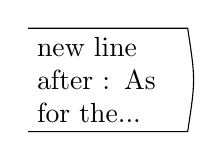
\begin{tikzpicture}\node[align=left,text width=1.8cm,inner sep=3pt] (n) {new line after : As for the...};\draw (n.north west)--(n.north east) .. controls ([xshift=1mm]n.east) .. (n.south east)--(n.south west);\end{tikzpicture}}}}
% The opposing pen brackets mark the paragraph break immediately before Quant au.
\handwritten{\tikz[baseline=-.6ex,scale=.18]{\draw (0,1.5)--(.5,1.4)--(.6,0)--(0,-.15);\draw (1.4,1.4)--(.9,1.35)--(.9,-.1)--(1.5,-.15);}}
As for the direct image functor $\mathrm{u}_{\handwritten{*}}$\inserted{$:\mathrm{E}\handwritten{\longrightarrow}\mathrm{E}'$}, which commutes with projective limits, it ``respects'' \inserted{therefore} every algebraic structure on an object (or a family of objects) of $\mathrm{E}$, definable in terms of projective limits \inserted{exclusively} (such as the str\deleted{i}uctures of a group, a ring or a module over a ring, \deleted{in}\inserted{among} the preceding examples). In \deleted{f}contrast, the functor $\mathrm{u}_{\handwritten{*}}$ is n\deleted{e}ot in general right exact i.e. it does not in general commute with finite inductive limits, and does not even in general transform epimorphism into epimorphism\handwritten{\unsure{;|,}} (it is moreover \deleted{\unsure{as} we shall see in the} this failure of exactness of the functor $\mathrm{u}_{\handwritten{*}}$ which is \handwritten{at} the source of these cohomological properties, which will be studied (from the point of view of commutative homological algebra) in the next lecture\handwritten{)}.
\inserted{\handwritten{Consequently, it does \deleted{not transform}\inserted{not extend}, in general,
\tikz[baseline=-.3ex,scale=.18]{\draw (0,0)--(.05,1.3) .. controls (-.35,1.65) and (.45,1.65) .. (.05,1.3);}
\figure{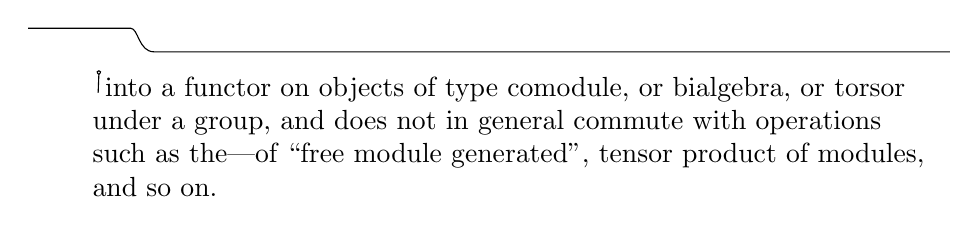
\begin{tikzpicture}
\node[inner sep=6pt,text width=.88\linewidth,align=left] (n) {\tikz[baseline=-.3ex,scale=.18]{\draw (0,0)--(.05,1.3) .. controls (-.35,1.65) and (.45,1.65) .. (.05,1.3);}into a functor on objects of type comodule, or bialgebra, or torsor under a group, and does not in general commute with operations such as \deleted{\unsure{the|of}} ``free module generated'', tensor product of modules, and so on.};
\draw ([xshift=-6mm,yshift=3mm]n.north west)--([xshift=7mm,yshift=3mm]n.north west) .. controls ([xshift=8mm,yshift=3mm]n.north west) and ([xshift=8mm]n.north west) .. ([xshift=10mm]n.north west)--(n.north east);
\end{tikzpicture}}}}

\deleted{2}\handwritten{3}.1.\handwritten{3}. In practice, when one \deleted{is given}\inserted{is \inserted{\handwritten{in}} the presence of} a functor $\mathrm{f}:\mathrm{E}\handwritten{\longrightarrow}\mathrm{F}$ from a $\underline{\mathrm{U}}$-topos to another, it is appropriate to make explicit \inserted{\handwritten{all}} its exactness proper\deleted{t}t\deleted{é}ies, \deleted{including and to determine whether it admits an exact functor} including the possible existence of left or right adjoint functors (cf. the preceding footnote), in order to arrive at an understanding of the ``geometric nature'' of $\mathrm{f}$, \deleted{which} an understanding which will generally be an indispensable guide for \deleted{the}\inserted{a} correct geometric intuition of the situation. Thus, if it turns out that $\mathrm{f}$ commutes with arbitrary inductive limits and with finite projective limits, it is appropriate to write $\mathrm{f}$ in the form
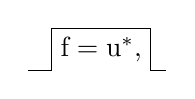
\begin{tikzpicture}[baseline=(n.base)]\node[inner sep=3pt] (n) {$\mathrm{f}=\mathrm{u}^{\handwritten{*}}$,};\handwritten{\draw ([xshift=-3mm]n.south west)--(n.south west)--(n.north west)--(n.north east)--(n.south east)--([xshift=2mm]n.south east);}\end{tikzpicture}
where
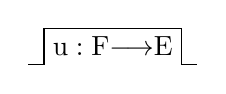
\begin{tikzpicture}[baseline=(n.base)]\node[inner sep=3pt] (n) {$\mathrm{u}:\mathrm{F}\handwritten{\longrightarrow}\mathrm{E}$};\handwritten{\draw ([xshift=-2mm]n.south west)--(n.south west)--(n.north west)--(n.north east)--(n.south east)--([xshift=2mm]n.south east);}\end{tikzpicture}
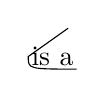
\begin{tikzpicture}[baseline=(n.base)]\node[inner sep=1pt] (n) {is a};\handwritten{\draw ([xshift=2mm,yshift=2mm]n.north)--(n.west) .. controls (n.south west) .. (n.south east);}\end{tikzpicture}
morphism of topoi, i.e. to interpret $\mathrm{f}$ as an ``inverse image'' functor by a ````continuous map'' of topoi. When $\mathrm{f}$ commutes with arbitrary projective limits, hence admits a left adjoint,\deleted{$\mathrm{g}$}
